\section{Hand pose estimation}
For the task of estimating the user's hand pose, two different hand pose regressors are implemented and evaluated.

For both regressors, ImageNetV2 \cite{Sandler} is implemented as an encoder to transfer the given depth data into a latent feature space. 

\subsection{Structural training}
As described in the previous section, the hand pose module uses an encoder to convert the high-dimensional input data into a latent feature space. 
Using the principle of transfer learning, the encoder can be trained separately in order to improve the overall performance of the pose regression network. This pretraining can involve any task which requires the encoder to transfer depth images of hands into some latent feature space.

Since depth images of human hands are prone to severe self-occlusion, they are hard to label precisely which limits the amount of available data. For the pretraining it is therefore preferable to train for a task which does not depend on potentially noisy labels. 

Training the encoder as part of an autoencoder is ideal under this circumstance since the target data is a direct copy (with some automatic modifications) of the input data. This simplifies the creation of additional training data.

On that basis an autoencoder is implemented, using MobileNetv2 \cite{Sandler} as its encoder part. With an input resolution of $224 \times 224$ pixels, the encoder transforms incoming depth maps into the latent feature space, consisting of $1280$ feature maps with a size of $7\times7$ each. 



The Autoencoder is trained on a custom dataset, consisting of short sequences of hand movements which are split into single frames. Its target is a segmented version of each depth map, containing only the hand and parts of the arm. 

In order to provide a wider range of backgrounds, a second dataset is then captured which contains no hands at all. By segmenting the hands from the first dataset and combining them with a random background from the second dataset, the variation of the dataset can be increased. Since the dataset consists exclusively of depth maps and the hand is guaranteed to be the closest object in each map, segmentation can be done by simply clipping values that are larger than a known threshold. The segmented hand images can then be used for both, the mentioned augmentation task and as the target for the autoencoder. 

\begin{figure}
	\centering
	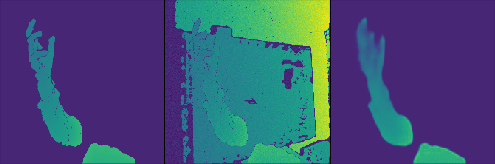
\includegraphics[width=0.7\linewidth]{Ressourcen/ae_example}
	\caption[Structural training]{Structural training. \textbf{Left}: Segmented depth map, containing only the hand and parts of the arm. \textbf{Center}: Segmented image with random background. \textbf{Right}: Reconstruction by the Autoenoder during training. }
	\label{fig:aeexample}
\end{figure}


 Additionally, classic augmentations methods like stretching, shearing and zooming/cropping are used to further augment the available data. As a final step, random noise is added to the input image, preserving 

\subsection{Training and Hyperparameter Tuning}


\section{Gesture Classification}
\section{Physical Construction}
